\documentclass[]{article}
\newcommand{\FileDepth}{../..}
\usepackage[a4paper, total={15cm,23cm}]{geometry}
\usepackage[T1]{fontenc}
\usepackage{textcomp}%Not strictly necessary, but gives \textmu command for "micro."
\usepackage{fancyhdr}
\usepackage{amsmath}
\usepackage{amssymb}
\usepackage{graphicx}
\usepackage{xcolor}
\usepackage{tikz}
\usetikzlibrary{calc}
\usepackage{cancel}%This is special for Activities 4 and 5.
%opening
\newcommand{\SecType}{X}
\newcommand{\Week}{X}
\title{Maximum Tilt}
\author{Benjamin Bauml}
\date{Spring 2024}
\pagestyle{fancy}
\rhead{PH 221}
\chead{Spring 2024}
\lhead{Week \Week}

% For Assignment, leave Purpose as 1. For Worksheet, set to 2. For Student Solution, set to 3. For Teacher Solution, set to 4.
% If you want keep the pieces from being called manually, set DefOnly to 0.
\newcommand{\Purpose}{4}
\newcommand{\DefOnly}{1}

% Version 2024-04-27
% Changes
% 2024-02-21 Added xstring package to enable smooth implementation of new \ModePage command.
% 2024-04-27 Set up to split activities and formatting aspects into separate files. Removed dependence on xcomment. Added an automatic counter to number the activities in a problem set.
\usepackage{tcolorbox}
\usepackage{xstring}
% You will want the following four lines in your document (the last two uncommented):
% For Assignment, leave Purpose as 1. For Worksheet, set to 2. For Student Solution, set to 3. For Teacher Solution, set to 4.
% If you want keep the pieces from being called manually, set DefOnly to 0.
%\newcommand{\Purpose}{4}
%\newcommand{\DefOnly}{1}
\newcommand{\Exclusion}{0}
\newcommand{\PageTurn}{0}
\newcommand{\GrayProb}{0}
\newcommand{\Tipsy}{0}

% Assignment
\if\Purpose1
\renewcommand{\Exclusion}{1}
\fi
% Worksheet
\if\Purpose2
\renewcommand{\Exclusion}{1}
\renewcommand{\PageTurn}{1}
\fi
% Student Solution
\if\Purpose3
\renewcommand{\PageTurn}{1}
\renewcommand{\GrayProb}{1}
\fi
% Teaching Copy
\if\Purpose4
\renewcommand{\PageTurn}{1}
\renewcommand{\GrayProb}{1}
\renewcommand{\Tipsy}{1}
\fi

\def \NewQ {0}
\def \PForce {0}
\newcommand{\MaybePage}[1]{
	\def \PForce {#1}
	\if\PForce1
	\newpage
	\else
	\if\NewQ0
	\gdef \NewQ {\PageTurn}
	\else
	\newpage
	\fi
	\fi
}

\newcommand{\ModePage}[1]{
	\IfSubStr{#1}{\Purpose}{\newpage}{}
}

\newcounter{ActNumber}
\setcounter{ActNumber}{0}

\newcommand{\Problem}[4][0]{%The first argument is optional, and if it is set to 1, the \newpage will be forced. The second argument is the name of the activity, the third is the command the activity is stored as, and the fourth is the actual problem statement.
\newcommand{#3}{
\MaybePage{#1}
\addtocounter{ActNumber}{1}
\section*{\SecType\Week-\theActNumber: #2}
\if\GrayProb1
\begin{tcolorbox}[colback=lightgray,colframe=lightgray,sharp corners,boxsep=1pt,left=0pt,right=0pt,top=0pt,bottom=0pt,after skip=2pt]
\else
\begin{tcolorbox}[colback=white,colframe=white,sharp corners,boxsep=1pt,left=0pt,right=0pt,top=0pt,bottom=0pt,after skip=2pt]
\fi
#4
\end{tcolorbox}\noindent
}
\if\DefOnly0
\else
#3
\fi
}
	
\newcommand{\ProblemSub}[3][0]{%The first argument is optional, and if a string of numbers is entered into it, it will force a \newpage in any \Purpose that shows up in the string. For example, "13" would lead to the newpage being forced in modes 1 and 3. The second is the command the activity is stored as, and the third is the actual problem statement.
\newcommand{#2}{
\ModePage{#1}
\if\GrayProb1
\begin{tcolorbox}[colback=lightgray,colframe=lightgray,sharp corners,boxsep=1pt,left=0pt,right=0pt,top=0pt,bottom=0pt,after skip=2pt]
\else
\begin{tcolorbox}[colback=white,colframe=white,sharp corners,boxsep=1pt,left=0pt,right=0pt,top=0pt,bottom=0pt,after skip=2pt]
\fi
#3
\end{tcolorbox}\noindent
}
\if\DefOnly0
\else
#2
\fi
}
		
\newcommand{\Solution}[2]{%The first argument is the command the solution is stored as, and the second is the actual solution.
\newcommand{#1}{
\if\Exclusion0
#2
\fi
}
\if\DefOnly0
\else
#1
\fi
}
		
\newcommand{\ProblemFig}[2]{%The first argument is the command the figure is stored as, and the second is the actual figure.
\newcommand{#1}{
\begin{figure}[h]
#2
\end{figure}
}
\if\DefOnly0
\else
#1
\fi
}
		
\newcommand{\TeachingTips}[1]{
\if\Tipsy1
\begin{tcolorbox}[colback=lightgray,colframe=black]
#1
\end{tcolorbox}
\fi
}

\newcommand{\FBDaxes}[3]{
	\begin{scope}[shift={(#1)},rotate=#2]
		% x-axis
		\draw[thick,->] (-2,0) -- (2,0);
		\node[anchor=west] at (2,0) {$x$};
		% y-axis
		\draw[thick,->] (0,-2) -- (0,2);
		\node[anchor=west] at (0,2) {$y$};
		\coordinate (#3) at (0,0);
	\end{scope}
}
\newcommand{\FBDvectorMA}[4]{
	\begin{scope}[shift={(#1)}]
		\coordinate (#4tip) at ({#2*cos(#3)},{#2*sin(#3)});
		\draw[ultra thick,blue,->] (#1) -- (#4tip);
	\end{scope}
}
\newcommand{\FBDvectorXY}[3]{
	\begin{scope}[shift={(#1)}]
		\coordinate (#3tip) at (#2);
		\draw[ultra thick,blue,->] (0,0) -- (#3tip);
	\end{scope}
}
\newcommand{\FBDdot}[1]{
	\filldraw[black] (#1) circle (3pt);
}

\begin{document}
\maketitle
\begin{center}
	This material is borrowed/adapted from PH 201 Tutorial 5 for Fall 2020 and Mastering Physics.
\end{center}

\Problem[1]{Maximum Tilt}{\MaximumTilt}{
A block is placed on an inclined plane and the angle of the plane is adjusted until the block just begins to slide. The coefficient of static friction is 0.35 and the coefficient of kinetic friction is 0.25.
}
\ProblemSub{\MaximumTiltA}{
(a) Draw a sketch illustrating the problem.
}
\Solution{\MaximumTiltASol}{
\begin{figure}[h]
	\centering
	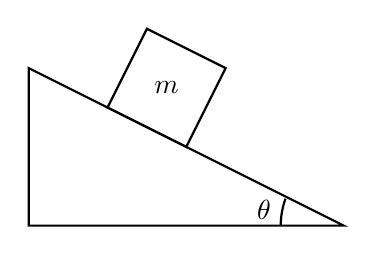
\begin{tikzpicture}
		\draw[thick] (0,0) -- (4,0) -- (0,2) -- cycle;
		\draw[thick] (3.2,0) arc (180:160:1);
		\node[anchor=east] at (3.2,0.2) {$\theta$};
		\draw[thick] (1,1.5) -- (2,1) -- (2.5,2) -- (1.5,2.5) -- cycle;
		\node at (1.75,1.75) {$m$};
	\end{tikzpicture}
\end{figure}
}
\ProblemSub{\MaximumTiltB}{
(b) Draw a free-body diagram for the block. Use the particle model with tilted axes.
}
\Solution{\MaximumTiltBSol}{
\begin{figure}[h]
	\centering
	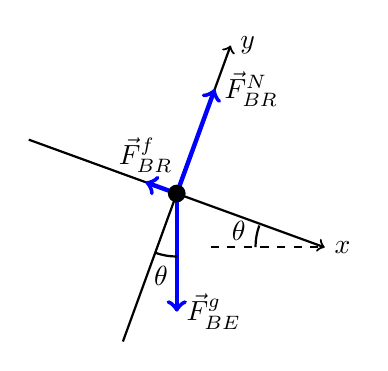
\begin{tikzpicture}
		\FBDaxes{0,0}{-20}{axes}
		\draw[thick,dashed] (1.8,-0.68) -- (0.4,-0.68);
		\draw[thick] (1,-0.68) arc (180:160:0.8);
		\node[anchor=east] at (1,-0.48) {$\theta$};
		\FBDvectorMA{axes}{1.41}{70}{FN}
		\node[anchor=west] at (FNtip) {$\vec{F}^{N}_{BR}$};
		\FBDvectorMA{axes}{0.42}{160}{FF}% 0.49 for static, 0.35 for kinetic
		\node[anchor=south] at (FFtip) {$\vec{F}^{f}_{BR}$};
		\FBDvectorXY{axes}{0,-1.5}{FG}
		\draw[thick] (0,-0.8) arc (270:250:0.8);
		\node[anchor=north] at (-0.2,-0.8) {$\theta$};
		\node[anchor=west] at (FGtip) {$\vec{F}^{g}_{BE}$};
		\FBDdot{axes}
	\end{tikzpicture}
\end{figure}

The diagram is qualitatively accurate for both the static and kinetic friction cases, though the friction vector may vary in size depending on which case we are looking at. Since there are no forces of the same type, I will drop the subscripts for the remainder of the problem (i.e. $F^{g}_{BE}$ will just be $F^{g}$, and so on).
}
\ProblemSub{\MaximumTiltC}{
(c) Find the angle at which the block just begins to slide.
}
\Solution{\MaximumTiltCSol}{
At the maximum angle for which the block doesn't slide, the force of static friction attains its maximum value. Tilting the surface even infinitesimally further, or giving the block the lightest push, will cause it to begin sliding. For now, both the $ x $ and $ y $ components of acceleration are zero. From the $ y $-components, we recover the normal force:
\[
\begin{split}
	F^{net}_{y} & = ma_{y} \\
	F^{N} + F^{g}_{y} & = 0 \\
	(F^{g}_{y} & = -mg\cos\theta) \\
	F^{N} & = -F^{g}_{y} = mg\cos\theta.
\end{split}
\]
This tells us that $ F^{sf}_{max} = \mu_{s}F^{N} = \mu_{s}mg\cos\theta $. We use this in the $ x $-component calculations:
\[
\begin{split}
	F^{net}_{x} & = ma_{x} \\
	F^{g}_{x} - F^{sf}_{max} & = 0 \\
	F^{sf}_{max} & = F^{g}_{x} = mg\sin\theta \\
	\mu_{s}\cancel{mg}\cos\theta & = \cancel{mg}\sin\theta \\
	\mu_{s} & = \frac{\sin\theta}{\cos\theta} = \tan\theta
\end{split}
\]
Now we can solve for the maximum angle:
\[
\theta = \arctan(\mu_{s}) = \arctan(0.35) \approx 19^{\circ} \text{ (2 sig figs)}.
\]
The maximum angle (accounting for significant figures) is 19$ ^{\circ} $, though we should carry the less approximate angle 19.3$ ^{\circ} $ through any further calculations.
}
\ProblemSub{\MaximumTiltD}{
(d) Keeping the angle the same, find the acceleration of the block after it starts to slide.
}
\Solution{\MaximumTiltDSol}{
Now, the friction is kinetic, and therefore it is smaller than the maximum static friction. This results in a net force and acceleration down the plane. The $ y $-component of acceleration is still zero, so we still have $ F^{N} = mg\cos\theta $. In the $ x $ direction, we have
\[
\begin{split}
	a_{x} & = \frac{1}{m} F^{net}_{x} \\
	& = \frac{1}{m} \left(F^{g}_{x} - F^{kf}\right) \\
	& = \frac{1}{m} \left(mg\sin\theta - \mu_{k} F^{N}\right) \\
	& = \frac{1}{m} \left(mg\sin\theta - \mu_{k} mg\cos\theta\right) \\
	& = g \left(\sin\theta - \mu_{k}\cos\theta\right) \\
	& = (9.8\text{ m/s}^{2})(\sin(19.3^{\circ}) - 0.25\cos(19.3^{\circ})) \\
	& \approx 0.93\text{ m/s}^{2}.
\end{split}
\]
}
\end{document}